\documentclass[11pt, a4paper, final]{report}

\usepackage[margin=1in, bottom=1in]{geometry}
\usepackage{amsmath}
\usepackage{graphicx}
\usepackage{amsfonts}
\usepackage{url}
\urlstyle{same}
\usepackage{titling}
\usepackage{lipsum}
\usepackage{setspace}
\usepackage{hyperref}
\usepackage{amsthm}

% boild math
\usepackage{bm}

\newcommand\onlyb[1]{\normalfont{\textbf{#1}}}
\newcommand\noSty[1]{\normalfont{#1}}
\newtheorem{theorem}{Teorema}[section]
\newtheorem{lemma}[theorem]{Lema}
\newtheorem{definition}[theorem]{Definisi}
\newtheorem{proposition}[theorem]{Proposisi}

% Bibliography stuffs i believe
\usepackage[bahasa]{babel}
\usepackage[fixlanguage]{babelbib}

% Bold extra
\usepackage{bold-extra}

% Image floating
\usepackage{float}

% Image subfigure
\usepackage{caption}
\usepackage{subcaption}

% Code highlight
\usepackage[newfloat]{minted}
\usepackage{xcolor} % to access the named colour LightGray
\definecolor{LightGray}{gray}{0.9}

% Pseudocode
\usepackage[ruled,linesnumbered]{algorithm2e}
\renewcommand*{\algorithmcfname}{Algoritma}
\SetKwInput{KwData}{Masukan}
\SetKwInput{KwResult}{Keluaran}

\usepackage{multirow}

% Separator length in itemize
\usepackage{enumitem}

\begin{document}
\begin{titlepage}
    \begin{center}\begin{figure}
            \begin{center}
                
\includegraphics[width=2.5cm]{makara.eps}
            \end{center}
        \end{figure}    
        \vspace*{0cm}
        \textbf{
        	UNIVERSITAS INDONESIA\\
        }
        
        \vspace*{1.0cm}
        % judul thesis harus dalam 14pt Times New Roman
        \textbf{Image Denoising} \\[1.0cm]
        
        \vspace*{3 cm}
        \textbf{Doki Doki Image Processing Club} \\
        % penulis dan npm


\begin{table}[H]
        \centering
        \begin{tabular}{c c}
            Eko Julianto Salim & 1906350925\\
            Hocky Yudhiono & 1906285604 \\
            Muhamad Nicky Salim & 1706039572\\
            Lucky Susanto & 1906350534\\
        \end{tabular}
        \end{table}
        \vspace*{5.0cm}

        % informasi mengenai fakultas dan program studi
        \textbf{
        	FAKULTAS ILMU KOMPUTER\\
        	DEPOK \\
        	DESEMBER 2021
        }
    \end{center}
\end{titlepage}

\onehalfspacing

\tableofcontents
\addcontentsline{toc}{chapter}{Daftar Isi}  

\begingroup
\listoffigures
\addcontentsline{toc}{chapter}{Daftar Gambar}  
\let\cleardoublepage\relax
\let\clearpage\relax
\listoftables
\addcontentsline{toc}{chapter}{Daftar Tabel}  
\endgroup

\chapter{Pendahuluan}

Data merupakan hal yang sangat diperlukan di masa ini. Data berguna pada hampir seluruh bidang sains, terutama untuk pemelajaran mesin. Namun, masalah terbesar dalam pembuatan model pemelajaran mesin yang bersifat \textit{state of the art} adalah data dalam jumlah besar.

Gambar merupakan salah satu jenis data yang sangat penting di bidang pemelajaran mesin dan dalam kehidupan sehari-hari. Dengan perkembangan di bidang ini, maka inovasi-inovasi seperti \textit{Real Time Sign Language Translation} hingga\textit{Autonomous Driving Car} dapat menjadi kenyataan. Beruntungnya, kita memiliki sangat banyak data dalam bentuk gambar. Salah satu cara pengambilan gambar yang sangat populer adalah melalui kamera \textit{smartphone} yang dimiliki oleh lebih dari setengah populasi manusia. Namun, pengambilan gambar secara konvensional ini memiliki masalah, yaitu \textit{noise}.

\textit{Noise} merupakan salah satu gangguan yang sulit dihindari saat melakukan pengambilan gambar. Menganalisis dan menghilangkan \textit{noise} dalam pengolahan citra merupakan salah satu langkah yang sangat sering dilakukan dalam bidang \textit{computer vision}. Hal ini dilakukan karena dalam melatih suatu model kecerdasan artifisial yang bisa digunakan dalam proses bisnis, \textit{noise} dapat menjadi salah satu faktor yang dapat mengurangi akurasi dan mengganggu proses \textit{training} suatu \textit{dataset}. Selain itu, proses pengolahan citra lain, misalnya dalam mempertajam gambar, butuh adanya \textit{denoising} atau \textit{noise removal} terlebih dahulu. Hal ini dikarenakan pengolahan \textit{image sharpening} dapat menyebabkan meningkatnya detail yang tidak diinginkan seperti \textit{noise}.

Ada banyak jenis \textit{noise} yang bisa muncul dalam suatu gambar, mulai dari \textit{gaussian}, \textit{salt and pepper}, \textit{banding}, \textit{periodic noise}, dan masih banyak lagi jenis yang dikategorikan oleh para peneliti dalam bidang \textit{computer vision}. Tidak ada metode \textit{image denoising} yang benar-benar dikatakan sempurna. Semua metode tersebut dapat mengurangi kualitas citra, sehingga informasi yang dapat diperoleh dari citra tersebut juga berkurang. Karena pada dasarnya proses ini merupakan imputasi data. Namun, pengurangan kualitas ini berbeda untuk setiap gambar dan metode \textit{image denoising} yang digunakan. Hal ini merupakan \textit{drawback} yang ingin dihindari dan menjadi pertimbangan bagi para pelaku industri maupun \textit{researcher} yang membutuhkan citra bebas \textit{noise} untuk diolah lebih lanjut.

\chapter{Isi}

Pada bab ini kami akan membahas mengenai eksperimen dan percobaan yang kami lakukan dalam melakukan \textit{image denoising}. Beberapa metode yang digunakan dalam laporan kami merupakan metode konvensional dan metode yang menggunakan pendekatan \textit{neural network} seperti \textit{vision transformer} yang sudah pernah dipublikasikan dalam jurnal \textit{computer vision}.

\section{Studi Literatur}

Ada banyak sekali \textit{noise} yang dapat terjadi dalam sebuah gambar. Dalam laporan ini, kami lebih fokus kepada \textit{noise} yang bersifat aditif karena cenderung muncul dalam citra dunia nyata, terutama yang disebabkan karena adanya disturbansi pada sinyal citra saat dilakukan perekaman oleh sensor.

Selama mata kuliah pengolahan citra, kita telah mempelajari berbagai kernel yang digunakan dalam melakukan konvolusi dan mentransformasi sebuah citra. Beberapa kernel seperti \textit{gaussian blur} dan \textit{average filter} yang umum digunakan untuk melakukan \textit{blurring} pada citra dapat menghilangkan \textit{noise}. Namun, filter ini juga melakukan \textit{smoothing} yang cenderung menghilangkan detail \textit{edge} yang cukup penting. Ada pula \textit{median filter} yang tidak linear dan menggunakan \textit{order statistics} dalam \textit{sliding box}-nya dan mentransformasikan citra baru berdasarkan mediannya. Filter ini cenderung menjaga \textit{edges} yang ada pada suatu gambar, namun kurang cocok untuk tipe \textit{noise} aditif.

\begin{figure}[H]
\centering
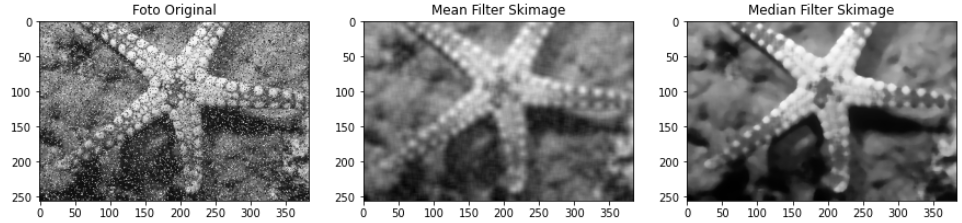
\includegraphics[scale=0.75]{assets/FilterKernel.png}
\caption{Filter Kernel}
\end{figure}

\subsection{Bilateral Filter}

Filter ini digunakan untuk \textit{smoothing} dan mengurangi \textit{noise} melalui nilai rata-rata dari nilai intensitas tetangganya, namun tetap menjaga detail sisi atau \textit{edges} yang terdapat pada citra dengan melibatkan bobot pada variasi intensitas di sekelilingnya. Dalam perhitungan dan rumusnya, \textit{bilateral filter} ini menggunakan \textit{gaussian filter} yang dimodifikasi.

\begin{figure}[H]
\centering
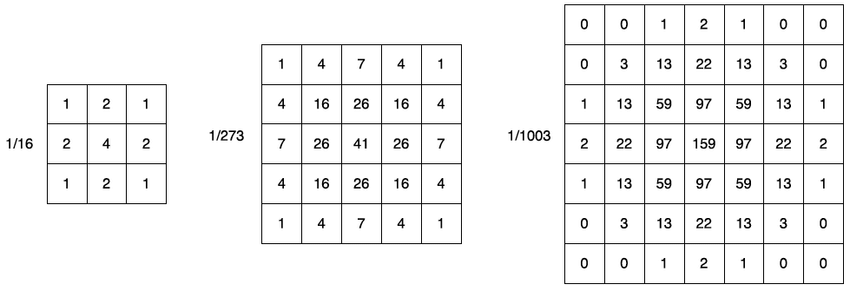
\includegraphics[scale=0.5]{assets/Gaussian.png}
\caption{Gaussian Blur Kernel \cite{gaussian}}
\end{figure}

\textit{Gaussian blur} dihitung menggunakan rumus sebagai berikut.

$$
GB[I]_p = \sum_{q \in S}{G_\sigma(||\vec{p} - \vec{q}||) I_q}
$$

$$
G_\sigma(||\vec{p} - \vec{q}||) = \exp(-{\frac{||\vec{p} - \vec{q}||^2}{\sigma^2}})
$$

Pada \textit{gaussian blur}, piksel yang berada di tengah ukuran kernel saat konvolusi memberikan kontribusi intensitas yang lebih tinggi terhadap piksel citra hasil transformasi. Sementara pada \textit{bilateral filter}, berlaku.

$$
BF[I]_p = \frac{1}{W^p} \sum_{q \in S}\underbrace{G_{\sigma_s}(||\vec{p}-\vec{q}||)}_{\text{\textit{terms} gaussian}}\underbrace{G_{\sigma_r}(||I_{p}-I_{q}||)}_{\text{\textit{terms} bias } I}I_q
$$
$$
W_p = \sum_{q\in S} G_{\sigma_s}(||\vec{p}-\vec{q}||)G_{\sigma_r}(||I_{p}-I_{q}||)I_q
$$

Perbedaan dari kedua filter ini terletak pada \textit{terms range intensity}-nya. Perhatikan ilustrasi berikut.

\begin{figure}[H]
\centering
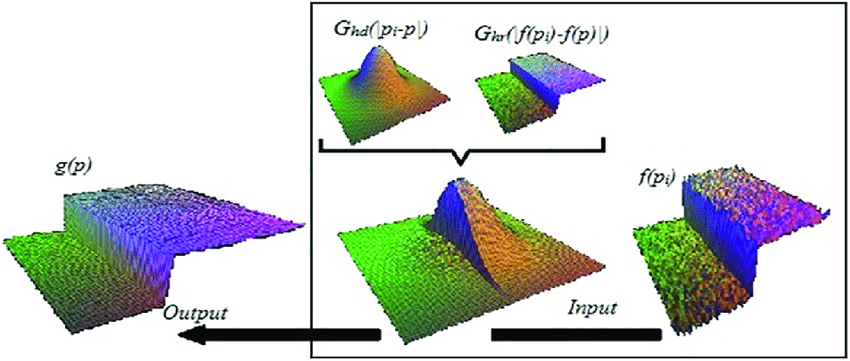
\includegraphics[scale=0.35]{assets/bilateralKernel.png}
\caption{Bilateral Filter Kernel \cite{ali2017soft}}
\end{figure}

\textit{Bilateral} filter ini merupakan perkalian antara kernel \textit{gaussian} dengan \textit{terms} perbedaan bias antar intensitas pada setiap \textit{channel}. Kernel baru yang dihasilkan merupakan dilatasi yang menyebabkan lebih tingginya kontribusi piksel yang berintensitas serupa dengannya. Dengan adanya kernel ini, maka \textit{edge} yang ditandai oleh perbedaan intensitas dapat tetap terjaga. Terdapat pula \textit{terms} $W_p$ yang merupakan normalisasi, sehingga gambar yang dihasilkan memiliki jangkauan dari $0$ hingga $1$. Untuk kompleksitas waktu dari \textit{gaussian blur} sendiri bisa linear, namun untuk \textit{bilateral filter} kompleksitas waktunya ialah $O(Nr^2)$ dengan $N$ ialah banyak pixel dan $r$ ialah ukuran jari-jari dari dari kernel yang didapat dari nilai $\sigma$ \cite{youtubeMaier}, seberapa jauh nilai kontribusi dari sebuah piksel membutuhkan piksel lain.

Terlepas dari performanya, berdasarkan observasi subjektif penulis, \textit{bilateral filter} ini sangat bagus dalam menghilangkan \textit{noise} yang bersifat aditif. Dalam praktiknya, nilai dari $\sigma_s$ dan $\sigma_r$ yang berturut-turut merupakan ukuran dari kernel \textit{gaussian} serta distribusi pengaruh dari perbedaan intensitas terhadap nilai akhir dari \textit{bilateral filter}. Semakin besar $\sigma_r$, maka akan semakin serupa dengan \textit{gaussian filter} biasa. Namun semakin kecil nilai $\sigma_r$ nya, maka \textit{noise} juga tidak akan hilang dan menjadi seperti gambar semula. Untuk menemukan konstanta yang pas, dibutuhkan percobaan secara subjektif dan/atau optimisasi pada metriks, serta pengaturan nilai yang tergantung dari resolusi dan konteks gambar.

\subsection{Guided Filter}

\textit{Guided filtering} merupakan salah satu alternatif atas \textit{bilateral filtering} yang ketika ukuran dari kernel semakin besar, maka biaya komputasinya juga akan membesar secara kuadratik. Kompleksitas waktu dari \textit{guided filtering} ini dengan implementasinya yang optimal ialah $O(N)$ \cite{he2015fast}. Guided filter bekerja dengan dua gambar masukan, gambar pertama ialah gambar yang ingin dijaga properti warnanya. Sementara gambar kedua ialah gambar yang menjadi \textit{guide} atau panduan untuk \textit{edges}-nya.

Misalnya dalam kasus saat mengambil gambar yang terang, detail warna yang masuk ke dalam sensor akan lebih banyak. Namun \textit{drawback}-nya ialah \textit{noise} yang didapatkan juga akan semakin banyak. Apabila kita memiliki satu gambar lain yang memiliki detail \textit{edge} yang lebih baik meskipun detail warna yang buruk --- (atau bahkan hitam putih), \textit{guided filter} memanfaatkan kedua gambar ini untuk mendapatkan gambar yang lebih baik. Gambar pertama disebut \textit{observed image} dan gambar kedua disebut \textit{guidance image}. Dalam praktiknya, filter ini sangat berguna dalam bidang medis. Selain itu, karena \textit{guided filter} berbasis persamaan linear, salah satu kekurangan dari \textit{bilateral filter} yang menyebabkan adanya \textit{gradient distortion} bisa diatasi dengan \textit{guided filter} yang tidak hanya menjaga \textit{edge}, namun juga menjaga \textit{gradient}.

\begin{figure}[H]
\centering
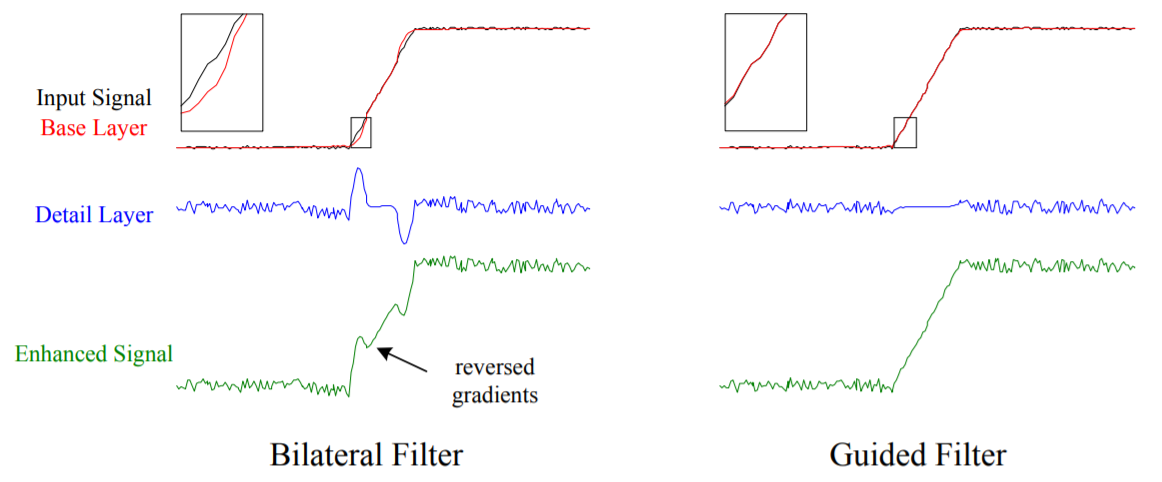
\includegraphics[scale=0.3]{assets/GradientDistortion.png}
\caption{Gradient Distortion \cite{he2015fast}}
\end{figure}

Definisikan $\bm{x}$ merupakan lokasi piksel yang ingin kita hitung intensitas nilai pada keluaran hasil \textit{filtering} ini, serta $i(\bm{x})$ dan $g(\bm{x})$ berturut-turut sebagai nilai dari intensitas \textit{guide image} dan \textit{observed image}. Keluaran dari gambar hasil \textit{filtering} diasumsikan merupakan kombinasi linear $f(\bm{x}')$ dari \textit{guide image}-nya dan sebuah konstanta.

$$
f(\bm{x}') = a_{\bm{x}} i(\bm{x}') + b_{\bm{x}}, \forall \bm{x}' \in \omega_{\bm{x}}
$$

Gradien dari persamaan ini akan didominasi oleh gambar \textit{guide} yang menjadi acuan \textit{edge}-nya, perhatikan bahwa $\nabla f = a \nabla i$. Selanjutnya, kita akan melakukan optimisasi, dengan \textit{cost function} $\mathcal{J}$ sebagai berikut.

$$
\mathcal{J}(a_{\bm{x}}, b_{\bm{x}}) = \sum_{\bm{x}'\in w_{\bm{x}}} (f(\bm{x}') - g(\bm{x}'))^2 + \epsilon a_{\bm{x}}^2
$$

$\epsilon$ merupakan konstanta regularisasi. Konstanta ini berguna agar nilai dari $a_{\bm{x}}$ atau kontribusi dari \textit{guide image}-nya tidak terlalu tinggi. Dengan melakukan turunan parsial terhadap $a_{\bm{x}}$ didapatkan persamaan sebagai berikut.

$$
\begin{aligned}
\frac{\partial}{\partial a_{x}} \mathcal{J}\left(a_{x}, b_{x}\right) &=\sum_{\boldsymbol{x}^{\prime} \in \omega_{x}}\left(\left(a_{x} i\left(\boldsymbol{x}^{\prime}\right)+b_{x}-g\left(\boldsymbol{x}^{\prime}\right)\right) i\left(\boldsymbol{x}^{\prime}\right)+\epsilon a_{x}\right) \stackrel{!}{=} 0 \\
\end{aligned}
$$

Selanjutnya bila dilakukan turunan parsial terhadap $b_{\bm{x}}$ didapatkan persamaan sebagai berikut.

$$
\begin{aligned}
\frac{\partial}{\partial b_{x}} \mathcal{J}\left(a_{x}, b_{x}\right) &=\sum_{\boldsymbol{x}^{\prime} \in \omega_{x}}\left(a_{\boldsymbol{x}} i\left(\boldsymbol{x}^{\prime}\right)+b_{\boldsymbol{x}}-g\left(\boldsymbol{x}^{\prime}\right)\right) \\
&=a_{\boldsymbol{x}} \sum_{\boldsymbol{x}^{\prime} \in \omega_{x}} i\left(\boldsymbol{x}^{\prime}\right)+b_{\boldsymbol{x}} \sum_{\boldsymbol{x}^{\prime} \in \omega_{x}} 1-\sum_{\boldsymbol{x}^{\prime} \in \omega_{x}} g\left(\boldsymbol{x}^{\prime}\right) \stackrel{!}{=} 0 \\
&=a_{\boldsymbol{x}} \sum_{\boldsymbol{x}^{\prime} \in \omega_{\boldsymbol{x}}} i\left(\boldsymbol{x}^{\prime}\right)+b_{\boldsymbol{x}}\left|\omega_{\boldsymbol{x}}\right|-\sum_{\boldsymbol{x}^{\prime} \in \omega_{\boldsymbol{x}}} g\left(\boldsymbol{x}^{\prime}\right) \stackrel{!}{=} 0 \\
b_{\boldsymbol{x}}&=\frac{1}{\left|\omega_{\boldsymbol{x}}\right|} \sum_{\boldsymbol{x}^{\prime} \in \omega_{\boldsymbol{x}}} g\left(\boldsymbol{x}^{\prime}\right)-a_{\boldsymbol{x}}\left(\frac{1}{\left|\omega_{\boldsymbol{x}}\right|} \sum_{\boldsymbol{x}^{\prime} \in \omega_{\boldsymbol{x}}} i\left(\boldsymbol{x}^{\prime}\right)\right)
\end{aligned}
$$

Untuk mencari nilai $a_{x}$ turunkan persamaan sebagai berikut.

$$
\begin{aligned}
a_{x}\left(\frac{1}{\left|\omega_{x}\right|} \sum_{x^{\prime} \in \omega_{x}} i\left(x^{\prime}\right) i\left(x^{\prime}\right)-\mathrm{E}_{\omega_{x}}[i(x)] \frac{1}{\left|\omega_{x}\right|} \sum_{x^{\prime} \in \omega_{x}} i\left(x^{\prime}\right)+\epsilon \frac{1}{\left|\omega_{x}\right|} \sum_{x^{\prime} \in \omega_{x}} 1\right) \\
=\frac{1}{\left|\omega_{x}\right|} \sum_{x^{\prime} \in \omega_{x}} g\left(x^{\prime}\right) i\left(x^{\prime}\right)-\mathrm{E}_{\omega_{\mathrm{m}}}[g(x)] \frac{1}{\left|\omega_{x}\right|} \sum_{x^{\prime} \in \omega_{x}} i\left(x^{\prime}\right) \\
\end{aligned}
$$

Beberapa persamaan tersebut bisa disederhanakan kembali dengan menyatakannya sebagai \textit{variance} dan \textit{covariance}.

$$
\begin{aligned}
\operatorname{Var}[X]&=\mathrm{E}\left[X^{2}\right]-\mathrm{E}[X]^{2} \\
\operatorname{Cov}[X, Y]&=\mathrm{E}[X Y]-\mathrm{E}[X] \mathrm{E}[Y] \\
\end{aligned}
$$
$$
\begin{aligned}
a_{\boldsymbol{x}}\left(\mathrm{E}_{\omega_{\boldsymbol{x}}}[i(\boldsymbol{x}) i(\boldsymbol{x})]-\mathrm{E}_{\omega_{\boldsymbol{x}}}[i(\boldsymbol{x})] \mathrm{E}_{\omega_{\boldsymbol{x}}}[i(\boldsymbol{x})]+\epsilon\right)&= \mathrm{E}_{\omega_{\boldsymbol{x}}}[g(\boldsymbol{x}) i(\boldsymbol{x})]-\mathrm{E}_{\omega_{\boldsymbol{x}}}[g(\boldsymbol{x})] \mathrm{E}_{\omega_{\boldsymbol{x}}}[i(\boldsymbol{x})] \\
a_{x}&=\frac{\operatorname{Cov}_{\omega_{x}}[g(\boldsymbol{x}), i(\boldsymbol{x})]}{\operatorname{Var}_{\omega_{\boldsymbol{x}}}[i(\boldsymbol{x})]+\epsilon} \\
\end{aligned}
$$

Saat nilai dari $i(\bm{x}) = g(\bm{x})$, berlaku persamaan sebagai berikut.
$$
\begin{aligned}
a_{\boldsymbol{x}}&=\frac{\operatorname{Var}_{\omega_{x}}(g(\boldsymbol{x}))}{\operatorname{Var}_{\omega_{x}}(g(\boldsymbol{x}))+\epsilon}\\
b_{\boldsymbol{x}}&=\mathrm{E}_{\omega_{\boldsymbol{x}}}(g(\boldsymbol{x}))-a_{\boldsymbol{x}} \mathrm{E}_{\omega_{\boldsymbol{x}}}(g(\boldsymbol{x}))
\end{aligned}
$$

Saat $\epsilon = 0$, maka jelas bahwa tidak ada filter yang terjadi. Perhatikan bahwa saat varians sangat rendah, dalam artian $g(\bm{x})$ nya mirip untuk suatu \textit{sliding windows}, maka $a_{\bm{x}}$ akan mendekati $0$, sehingga $b_{\bm{x}}$ akan mendekati $\mathrm{E}_{\omega_{\boldsymbol{x}}}(g(\bm{x}))$. Sebaliknya, saat variansinya tinggi, maka nilai $\epsilon$ akan semakin tidak berguna karena ditutupi oleh variansi, sehingga $a_{\bm{x}}$ akan mendekati $1$ dan $b_{\bm{x}}$ akan mendekati $0$. Hal ini menandakan adanya \textit{edge}, sehingga \textit{guide image} akan dipertahankan. Perhatikan bahwa definisi filter ini pada akhirnya ialah sebagai berikut.

$$
f_{\mathrm{GF}}(\boldsymbol{x})=\frac{1}{\left|\omega_{\boldsymbol{x}^{\prime}}\right|} \sum_{\boldsymbol{x}^{\prime}: \boldsymbol{x} \in \omega_{\boldsymbol{x}^{\prime}}}\left(a_{\boldsymbol{x}^{\prime}} i(\boldsymbol{x})+b_{\boldsymbol{x}^{\prime}}\right)=\mathrm{E}_{\omega_{\boldsymbol{x}^{\prime}}}\left[a_{\boldsymbol{x}}\right] i(\boldsymbol{x})+\mathrm{E}_{\omega_{\boldsymbol{x}^{\prime}}}\left[b_{\boldsymbol{x}}\right]
$$

Perhatikan bahwa ukuran dari kernel serta nilai $\epsilon$ merupakan parameter yang harus disesuaikan dengan gambar pula \cite{youtubeMaier}.

Selain dari segi kompleksitas waktu, guided filter memiliki keuntungan atas masalah dari bilateral filter, yaitu adanya kemungkinan \textit{gradient reversal}, yaitu meskipun \textit{edges}-nya ter-\textit{maintain}, tapi gradiennya tidak, beda halnya dengan \textit{guided filter} ini \cite{guidedFilter}. Menghitung nilai dari $a_{\bm{x}}$ dan $b_{\bm{x}}$ akan sangat mudah dengan melakukan \textit{prefix-sum 2D} dengan \textit{dynamic programming}. 

\subsection{Non-Local Means Denoising Filter}

Berbeda dengan kedua metode sebelumnya, metode ini tidak bersifat lokal. Filter ini memanfaatkan keseluruhan gambar sebagai nilai yang dapat berkontribusi atas keluarannya. Cara kerjanya cukup sederhana, yaitu mencari rata-rata dari seluruh piksel dalam gambar dengan memberikan bobot koefisien dengan suatu nilai distribusi, umumnya \textit{gaussian} dari keserupaan suatu \textit{patch} atau \textit{windows} \cite{buades2011non}.

$$
f(\bm{x}) = \frac{1}{z} \sum_{\bm{x}' \in X} G_\sigma (N_{\bm{x}} - N_{\bm{x}'}) g(\bm{x})
$$

Perhatikan bahwa $N_{\bm{x}}$ merupakan suatu \textit{windows} yang berpusat pada $\bm{x}$. Nilai dari $N_{\bm{x}} - N_{\bm{x}'}$ umumnya akan dihitung \textit{norm}-nya, kemudian akan dicari nilai dari $G_\sigma$-nya. $z$ merupakan \textit{terms} normalisasi. Perhatikan juga terdapat beberapa variasi dari $X$. Pada umumnya $X$ merupakan himpunan setiap piksel pada gambar. Namun bisa saja $X$ juga merupakan sebuah \textit{windows} yang tentunya ukurannya harus lebih besar dari besar dari ukuran matriks $N$. Kompleksitas waktu untuk filter ini cukup tinggi, yaitu $O(N^2 r^2)$ dengan $r$ ialah ukuran dari \textit{windows} yang diparameteri oleh $\sigma$.

\subsection{Deep Learning Method and Image Transformer}

\subsubsection{Convolutional Neural Network}

\textit{Convolutional Neural Network} adalah sebuah model \textit{neural network} yang bekerja dengan cara melakukan operasi konvolusi terhadap gambar input. Konvolusi adalah proses pemetaan nilai sebuah daerah pada gambar menjadi hanya satu nilai saja. Hal ini diulang berkali-kali sehingga semua daerah pada gambar telah dikonvolusikan.

\begin{figure}[H]
\centering
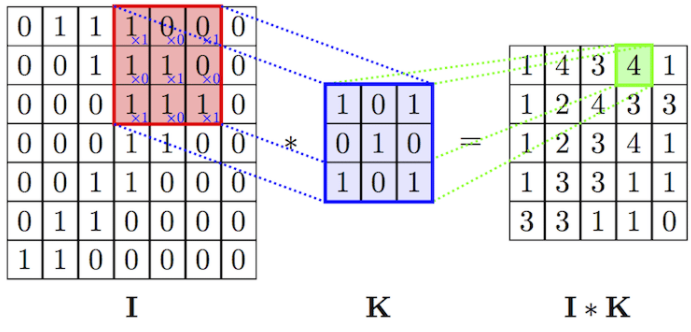
\includegraphics[scale=0.6]{assets/convolution.png}
\caption{Ilustrasi Konvolusi \cite{deepl2021}}
\end{figure}

Kelebihan dari model yang CNN ini adalah simplisitasnya dan tingkat akurasinya yang sangat tinggi. Kedua kelebihan ini menyebabkan model CNN sebagai sebuah model yang sangat sering digunakan oleh banyak orang dalam bidang pengolahan citra dan \textit{computer vision}. Namun, model ini tetaplah memiliki banyak kekurangan yang bisa diperbaiki.

Proses konvolusi memiliki beberapa kelemahan. Sebagai sebuah ilustrasi, jika kita menggunakan konvolusi berukuran $3 \times 3$, maka hasil konvolusinya dipengaruhi oleh $9$ buah piksel. Satu piksel dan 8 buah piksel tetangganya. Karena sifat ini, sebuah \textit{feature map} yang didapatkan melalui konvolusi bersifat lokal tanpa mempedulikan properti global \textit{input}-nya. Hal ini ditakutkan dapat meningkatkan bias.

\subsubsection{Attention Mechanism}

Kelemahan dari CNN menyebabkan orang mencari cara lain yang menghasilkan \textit{feature map} yang bersifat non-lokal. Oleh karena itu, masuklah \textit{Attention Mechanism} ke bidang \textit{Image Processing} yang awalnya berasal dari bidang \textit{Machine translation}. 

\begin{figure}[H]
\centering
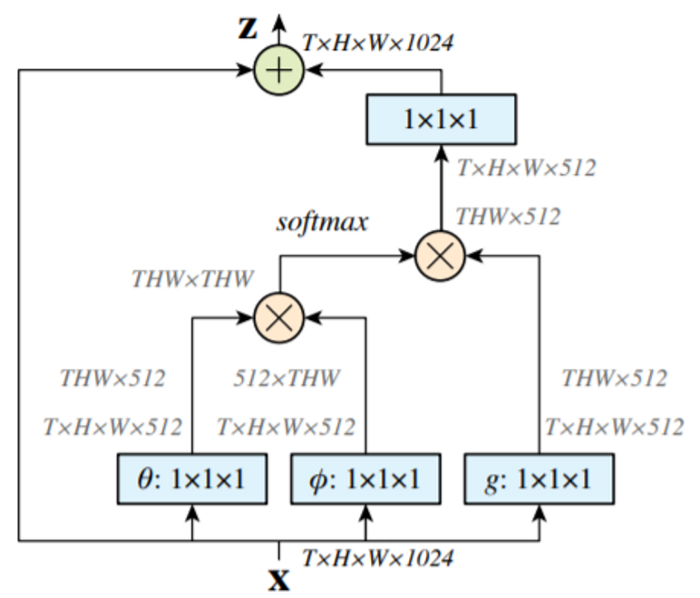
\includegraphics[scale=0.25]{assets/AttentionModel.png}
\caption{Ilustrasi Model Attention \cite{wang2018nonlocal}}
\end{figure}

\textit{Attention Mechanism} mengikuti konsep kovarian yang terdapat di statistik. Kovarian sendiri memberikan gambaran mengenai seberapa mirip persebaran dari suatu variabel acak dari variabel acak lainnya. Kovarian lalu akan bersifat menjadi \textit{weight} dari setiap piksel pada masukan. Perhatikan bahwa melalui penggunaan \textit{attention mechanism}, ukuran dari keluaran sama dengan ukuran dari masukan kita. Karena setiap piksel pada keluaran merupakan penjumlahan dari piksel masukan yang sudah diberi \textit{weight}, maka sifat non-lokal pun dapat tercapai.

\begin{figure}[H]
\centering
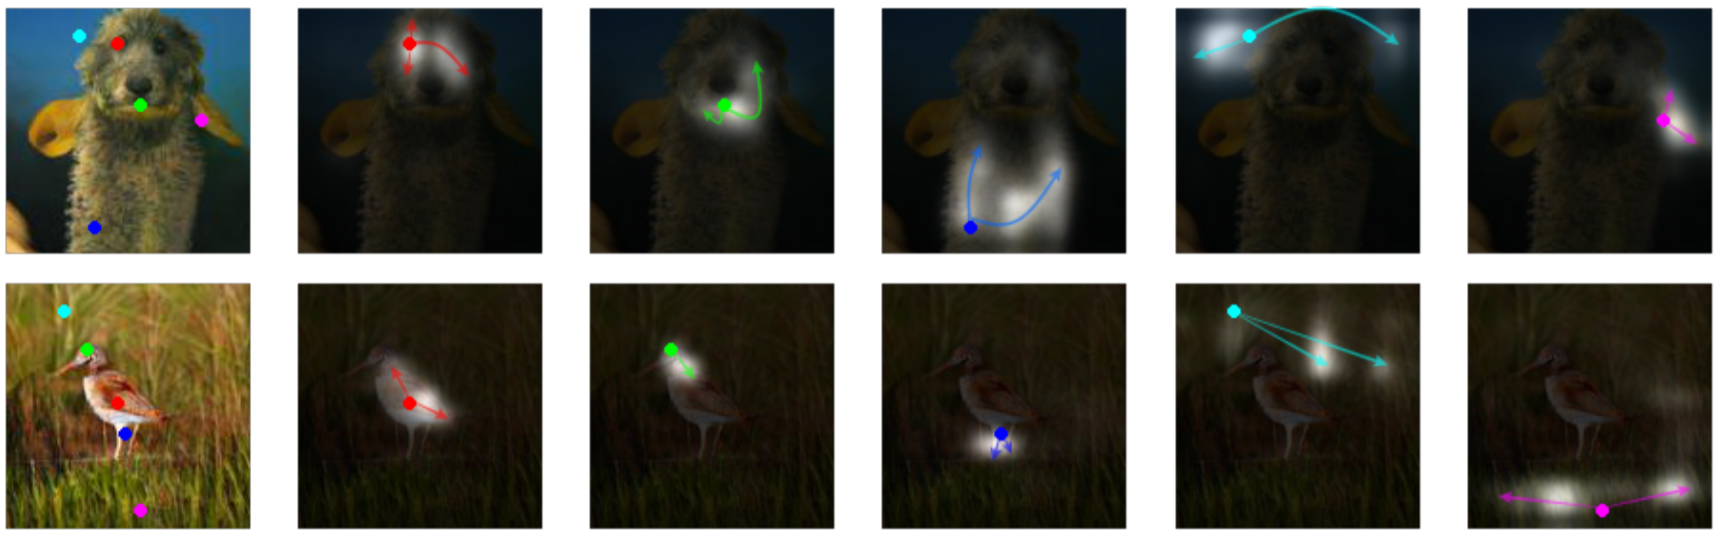
\includegraphics[scale=0.4]{assets/AttentionModel2.png}
\caption{Sifat Non-Lokal Model Atensi \cite{zhang2019selfattention}}
\end{figure}

\subsubsection{Vision Transformer}

Dulunya state-of-the-art dari permasalahan pengolahan citra didominasi oleh CNN, namun sebuah Vision Transformer (ViT) bisa memberikan hasil klasifikasi yang lebih baik saat \textit{training dataset} yang diberikan cukup banyak \cite{dosovitskiy2021image}. ViT dibuat berdasarkan \textit{transformer} yang biasanya digunakan dalam Natural Language Processing (NLP) \cite{vaswani2017attention}.

Vision Transformer ini merupakan salah satu metode \textit{deep learning} yang menggunakan mekanisme \textit{Attention}. Untuk data yang lebih sedikit, \textit{bias}-nya cukup rendah sehingga butuh regularisasi dan augmentasi data. Setiap gambar awalnya akan dibagi menjadi beberapa bagian yang disebut \textit{patch}. Dalam NLP, layaknya kalimat yang dijadikan kumpulan kata-kata. CNN membutuhkan sumber daya empat kali lebih besar untuk mendapatkan performa yang setara dengan sebuah Vision Transformer. Dalam komputasinya CNN membutuhkan kumpulan piksel-piksel, sementara ViT membaginya menjadi sekumpulan token-token. Layer Self-Attention dalam ViT memberikan konteks secara global untuk seluruh gambar meskipun dibagi-bagi tadi gambarnya. Selain itu, model tersebut juga mengetahui lokasi dari masing-masing \textit{patch} untuk menyusun ulang struktur dari sebuah citra.

Sebuah \textit{transformer encoder} memiliki:
\begin{itemize}[noitemsep]
    \item Multi-Head Self Attention Layer (MSP) yang menggabungkan semua \textit{output attention} pada dimensi yang benar, membantu \textit{training} secara lokal dan global.
    \item Multi-Layer Perceptrons (MLP) Layer yang di dalamnya terdapat dua layer Gaussian Error Linear Unit (GELU)
    \item Layer Norm (LN) ditambahkan karena tidak ada dependensi tambahan antara setiap citra yang akan digunakan untuk \textit{training}. \textit{Layer} ini meningkatkan waktu dan performa.
\end{itemize}

\begin{figure}[H]
\centering
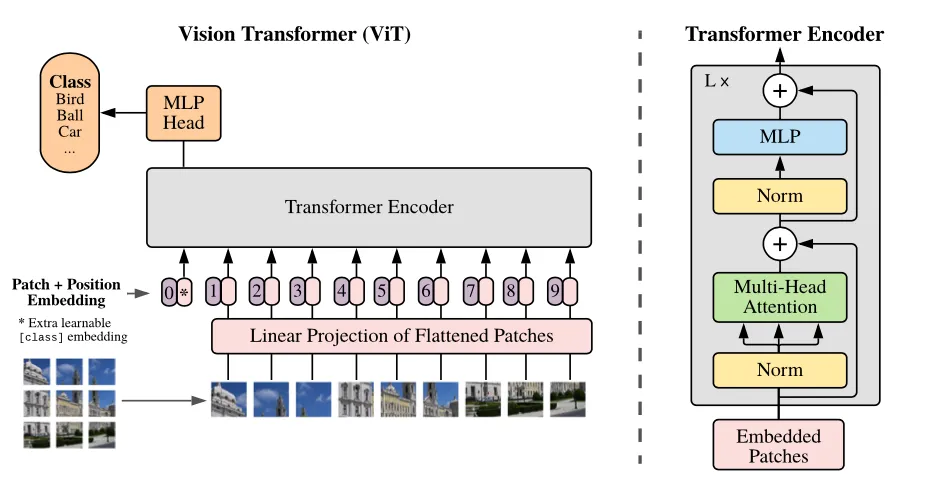
\includegraphics[scale=0.5]{assets/ViT.png}
\caption{Arsitektur Vision Transformer \cite{dosovitskiy2021image}}
\end{figure}

Secara umum, sebuah \textit{vision transformer} akan bekerja:
\begin{itemize}[noitemsep]
    \item Membagi gambar menjadi beberapa \textit{patch} yang ukurannya sama
    \item Menjadikannya matriks kolom
    \item Membuat \textit{linear embedding} yang pada dasarnya melakukan reduksi dimensi.
    \item Menambahkan \textit{positional embedding}
    \item Memasukkannya ke dalam \textit{transformer encoder}
    \item Lakukan \textit{training} dan \textit{tuning} seperti biasa.
\end{itemize}

\subsubsection{Uformer}


\begin{figure}[H]
\centering
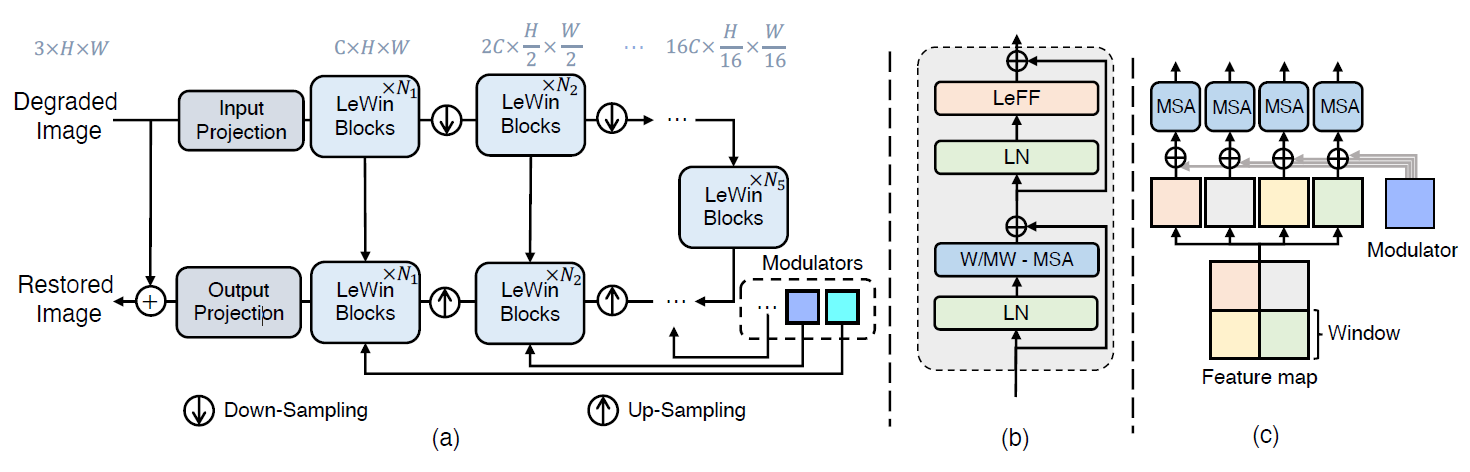
\includegraphics[scale=0.5]{assets/Uformer.png}
\caption{Arsitektur Uformer \cite{dosovitskiy2021image}}
\end{figure}

Arsitektur ini dibuat berdasarkan arsitektur U-Net, yang layer-layer konvolusinya digantikan dengan blok-blok transformer. Dalam kasus ini, digunakan Locally-enhanced Window (LeWin) \textit{transformer block} yang membuat \textit{self-attention}-nya terbatas dalam suatu \textit{window} tertentu, dan tidak global, sehingga bisa mengurangi kompleksitas komputasi untuk \textit{feature maps} yang banyak. Kemudian juga ada \textit{multi-scale} modulator yang digunakan untuk memperbaiki gangguan dan kecacatan pada gambar.

\subsubsection{Restormer}

\begin{figure}[H]
\centering
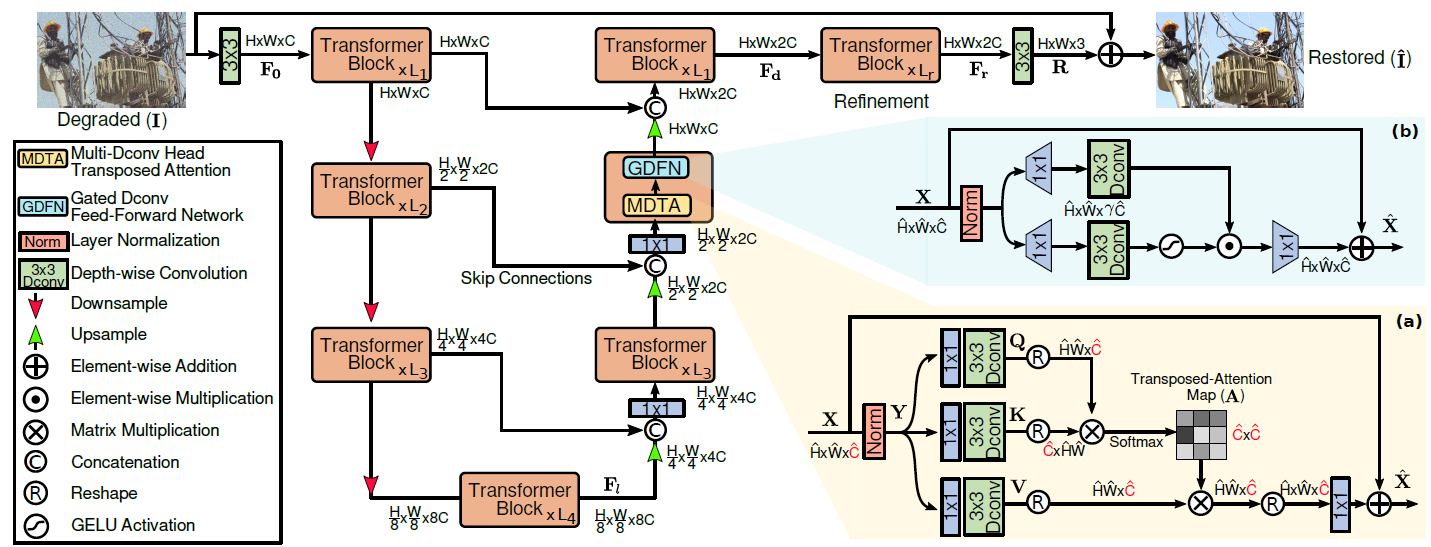
\includegraphics[scale=0.5]{assets/Restormer.png}
\caption{Arsitektur Restormer \cite{dosovitskiy2021image}}
\end{figure}

Restormer merupakan transformer yang bentuknya \textit{encoder-decoder} juga untuk memanfaatkan representasi lokal dan globalnya. Ada pula modul yang dinamakan multi-Dconv head transposed attention (MDTA) yang mampu mencari hubungan dan/atau interaksi antar piksel lokal dan non-lokal.. Ada pula gated-Dconv feed-forward network (GDFN) yang menyaring agar hanya fitur-fitur yang informatif saja yang masuk ke jaringan.

\subsection{Denoising Metrics}

Dalam mengukur tingkat akurasi kualitas suatu gambar, dibutuhkan suatu standar yang bisa digunakan untuk membandingkan dua buah hasil citra. Dalam melakukan \textit{assessment}, terdapat metode objektif yang biasanya direpresentasikan secara numerik. Namun tentu saja, tujuan akhir dari pengolahan suatu citra ialah untuk observasi berdasarkan \textit{visual pleasingness} manusia. Sehingga metode objektif ini sebisa mungkin ingin dapat menilai suatu citra secara numerik namun tetap sebanding dengan penilaian oleh manusia secara subjektif.

Karena dataset yang kita miliki memiliki \textit{ground truth}, melakukan \textit{assessment} secara \textit{full-reference} atau membandingkannya secara langsung dengan citra yang dianggap benar dapat memberikan hasil yang lebih \textit{reliable} dan tidak ada ambiguitas. Salah satu metriks sederhana yang umum digunakan ialah \textit{Mean Square Error} yang pada dasarnya merupakan perbandingan norm antar matriks kolom dari kedua gambar. \textit{Mean Square Error} dapat dihitung menggunakan rumus sebagai berikut.

$$
MSE = \frac{\sum_{m \in M, n \in N}((I(m, n) - J(m, n))^2}{M \cdot N}
$$

Salah satu metriks MSE based yang digunakan oleh kami ialah \textit{Peak Signal to Noise Ratio} (PSNR) yakni sebagai berikut.

$$
PSNR = 10 \log_{10} \frac{R^2}{MSE}
$$

Dengan $R$ merupakan nilai intensitas maksimum yang terdapat pada gambar, pada gambar yang direpresentasikan oleh bilangan bulat tak bertanda berukuran 8-bit, $R = 255$, bila gambar direpresentasikan oleh \textit{floating point} dalam interval $[0, 1]$ maka $R = 1$. Perhatikan bahwa semakin besar $MSE$, maka akurasi dianggap semakin buruk. Oleh karena itu, semakin besar $PSNR$, yang artinya $MSE$ semakin mendekati $0$, maka kualitas gambar dianggap menjadi semakin baik. PSNR biasanya digunakan untuk mengukur kualitas gambar hasil kompresi. Dalam kasus ini, \textit{noise} yang muncul biasanya karena adanya kompresi itu sendiri.

Selain itu, ada pula metriks pengukuran berdasarkan struktur dari citra. Salah satu yang kami gunakan ialah \textit{Structural imilarity} (SSIM). SSIM merupakan pengganti dari Universal Quality Index (UQI). SSIM mempertimbangkan tiga parameter, yaitu \textit{luminance}, kontras, dan struktur dari sebuah gambar. Nilai dari SSIM dapat dihitung menggunakan rumus berikut.

$$
\begin{aligned}
l(x, y)&=\frac{2 \mu_{x} \mu_{y}+c_{1}}{\mu_{x}^{2}+\mu_{y}^{2}+c_{1}} \\
c(x, y)&=\frac{2 \sigma_{x} \sigma_{y}+c_{2}}{\sigma_{x}^{2}+\sigma_{y}^{2}+c_{2}} \\
s(x, y)&=\frac{\sigma_{x y}+c_{3}}{\sigma_{x} \sigma_{y}+c_{3}} \\
c_{3}&=c_{2} / 2 \\
\operatorname{SSIM}(x, y)&=\left[l(x, y)^{\alpha} \cdot c(x, y)^{\beta} \cdot s(x, y)^{\gamma}\right]
\end{aligned}
$$

Dalam praktiknya, $\alpha, \beta, \gamma$ bernilai $> 0$ dan akan disesuaikan berdasarkan kontribusi dan kepentingan masing-masing komponen. Saat nilai ketiganya $= 1$, maka didapatkan rumus sebagai berikut.

$$
\operatorname{SSIM}(x, y)=\frac{\left(2 \mu_{x} \mu_{y}+c_{1}\right)\left(2 \sigma_{x y}+c_{2}\right)}{\left(\mu_{x}^{2}+\mu_{y}^{2}+c_{1}\right)\left(\sigma_{x}^{2}+\sigma_{y}^{2}+c_{2}\right)}
$$

Dengan $\mu$ merupakan rata-rata dan $\sigma$ merupakan variansi. Untuk menghitung nilai SSIM pada seluruh gambar, dihitung rata-rata untuk setiap piksel dan nilainya dinormalisasi di antara $[0, 1]$ semakin tinggi nilai SSIM, maka sebuah citra dianggap memiliki gambar dengan kualitas yang lebih baik.

 \section{Desain Eksperimen}

Pada eksperimen yang kami lakukan, kami menggunakan 40 citra berwarna dalam ruang citra RGB dari dataset \hyperlink{https://github.com/csjunxu/PolyU-Real-World-Noisy-Images-Dataset}{PolyU: Real-world Noisy Image Denoising}. Citra tersebut dibagi menjadi $100$ potongan yang masing-masing berukuran $512 \times 512$. Gambar-gambar tersebut diambil dengan berbagai kamera digital dan mengandung citra yang beragam dari segi intensitasnya. Terdapat gambar asli dan gambar \textit{ground truth} yang diperoleh dari rata-rata $500$ pengambilan gambar yang telah diseleksi secara manual \textit{outlier}-nya, kemudian disatukan dengan mengambil rata-rata dari piksel setiap gambar \cite{xu2018realworld}.

\textit{Ground truth} ini diasumsikan dapat merepresentasikan citra yang sesungguhnya terlepas dari gangguan dan faktor lain seperti \textit{blur} atau pun kualitas gambar yang tidak tajam. Untuk proses pengambilan gambar dan tolak ukur \textit{PolyU dataset} terhadap beberapa metode \textit{denoising} dengan metriks SSIM dan PSNR dapat dilihat pada jurnal tersebut. Dalam laporan ini, kami akan membandingkan beberapa metode konvensional yang umum digunakan, serta metode-metode \textit{deep learning} yang merupakan \textit{state-of-the-art} saat penulis menuliskan laporan ini. Metode-metode yang kami gunakan antara lain sebagai berikut.

\begin{itemize}[noitemsep]
    \item \textit{Non-Local Means Denoising Filter}
    \item \textit{Bilateral Filter}
    \item \textit{Guided Filter}
    \item \textit{Restormer: Efficient Transformer for High Resolution Image Restoration}
    \item \textit{Uformer: A General U-Shaped Transformer for Image Restoration}
\end{itemize}

Dataset dibagi menjadi $32$ untuk melatih model \textit{deep learning} dan $68$ untuk validasi, sekaligus mengevaluasi dan membandingkan antar metode. Data citra yang digunakan untuk pelatihan ialah dengan awalan sebagai berikut.

\begin{itemize}[noitemsep]
    \item \texttt{Sony\_4-5\_125\_3200\_plant}
    \item \texttt{Canon5D2\_5\_160\_6400\_reciever}
    \item \texttt{Canon5D2\_5\_160\_6400\_bicycle}
    \item \texttt{NikonD800\_4-5\_160\_1800\_classroom}
    \item \texttt{NikonD800\_8\_100\_6400\_bulletin}
    \item \texttt{Canon5D2\_5\_160\_6400\_circuit}
    \item \texttt{Canon5D2\_5\_200\_3200\_fruit}
    \item \texttt{NikonD800\_5\_100\_4000\_flower}
\end{itemize}

Sisanya digunakan sebagai validasi. Untuk Uformer dan Restormer dilakukan $8$ buah augmentasi yang melibatkan rotasi dan \textit{flip}, digunakan juga \textit{transfer learning} menggunakan checkpoint \textit{pretrained weights} yang terdapat pada repositori penulis Uformer, yaitu \texttt{uformer16\_denoising\_sidd.pth} dan serupa juga untuk Restormer \cite{wang2021uformer}. Selain itu karena keterbatasan sumber daya dan limitasi model, pelatihan model Restormer tidak bisa menggunakan citra berukuran 512x512. Maka dari itu, diberlakukan \textit{progressive training} dengan menggunakan citra hasil \textit{randomized cropping} untuk ukuran crop 256x256 dan 384x384 untuk Restormer (dan dilanjutkan citra awal 512x512 untuk Uformer).

Kode eksperimentasi dijalankan pada platform Google Cloud Vertex AI Workbench menggunakan instance \texttt{a2-highgpu-1g} (12vCPU, 85GB RAM, 1xA100) dan menggunakan \textit{library} Pytorch, Pytorch Lightning, Skimage dan OpenCV.

\section{Hasil dan Analisis}

Menggunakan \textit{grid search} untuk mencari tahu parameter yang pas untuk \textit{bilateral} dan \textit{guided filter}. Pada \textit{guided filter} didapatkan parameter $radius = 2$ dan $\epsilon = 250$ yang menghasilkan PSNR dan SSIM optimal. Pada bilateral filter, didapatkan parameter $\sigma_c = 2$ dan $\sigma_s = 3$. Didapatkan hasil dari $100$ potongan gambar berukuran $512 \times 512$ sebagai berikut.

\begin{table}[H]
\centering
\begin{tabular}{|c|c|cccc|cc|}
\hline
Jenis                   & \multirow{2}{*}{Noisy} & \multicolumn{4}{c|}{Konvensional}                                                                            & \multicolumn{2}{c|}{Deep Learning}         \\ \cline{1-1} \cline{3-8} 
Metode                  &                               & \multicolumn{1}{c|}{Bilateral} & \multicolumn{1}{c|}{NL Means}  & \multicolumn{1}{c|}{Guided}    & Wavelet   & \multicolumn{1}{c|}{\textbf{Uformer}}   & Restormer \\ \hline
Waktu (s) & -                             & \multicolumn{1}{c|}{$269$}     & \multicolumn{1}{c|}{$40.8$}    & \multicolumn{1}{c|}{$\mathbf{1.59}$}    & $8.09$    & \multicolumn{1}{c|}{$8.65$}    & $17.9$    \\ \hline
PSNR (dB)               & $36.4984$                     & \multicolumn{1}{c|}{$37.7612$} & \multicolumn{1}{c|}{$37.8896$} & \multicolumn{1}{c|}{$38.3948$} & $36.4999$ & \multicolumn{1}{c|}{$\mathbf{39.7207}$} & $39.5533$ \\ \hline
SSIM                    & $0.9097$                      & \multicolumn{1}{c|}{$0.9484$}  & \multicolumn{1}{c|}{$0.9530$}  & \multicolumn{1}{c|}{$0.9587$}  & $0.9098$  & \multicolumn{1}{c|}{$\mathbf{0.9702}$}  & $0.9697$  \\ \hline
\end{tabular}
    \caption{Hasil Evaluasi Komputasi}
\end{table}

Dari penilaian \textit{speed}, \textit{bilateral filtering} kecepatannya sangat dipengaruhi pada parameter. Karena semakin besar $\sigma$ yang diberikan, maka komputasi yang dilakukan akan semakin lama. Dalam kasus ini, $\sigma$ masih dianggap kecil. Menggunakan mesin komputasi yang sama, dengan performa yang optimal untuk setiap filter, waktu yang dibutuhkan untuk melakukan \textit{bilateral filtering} lima kali lebih lambat dibandingkan \textit{guided filtering}. Saat melakukan \textit{grid search parameter} pula, \textit{guided filtering} memberikan waktu yang serupa dalam menghitung hasil \textit{filtering}-nya untuk setiap nilai parameter $\sigma$ dan $\epsilon$ yang berbeda. Untuk $\sigma_c = \sigma_s = 5$ pada saat melakukan \textit{grid search}, dibutuhkan waktu sekitar $12.5$ kali lebih lambat dibandingkan \textit{guided filtering}.

Untuk \textit{non-local means} sendiri memberikan waktu yang paling lambat dalam performanya yang optimal. Hal ini karena dibutuhkannya komputasi yang cukup banyak dalam setiap iterasi pikselnya. Untuk gambar yang banyak atau ukuran yang lebih besar, tentunya metode ini tidak \textit{scalable} karena kompleksitas waktunya yang sangat bergantung pada banyak piksel. Secara teori, sekitar $O(N^2)$ komputasi. Berbeda dengan $O(N)$ pada \textit{guided filtering} dan $O(Nr^2)$ pada \textit{bilateral filtering}. Dari segi \textit{scalability}, tentunya metode \textit{guided filtering} sangat unggul.

Untuk penilaian secara subjektif dan \textit{interpretability}-nya, penulis memberikan perbandingan antara gambar original, bilateral, guided, non-local means dan \textit{ground truth} kepada beberapa narasumber anonim dan menanyakan gambar mana yang menurut narasumber paling \textit{eyepleasing} dan bagus dalam menghilangkan \textit{noise}. Secara umum, hasil yang memberikan kesan secara subjektif ialah yang \textit{non-local means} dan \textit{guided filtering}. Keduanya tidak selalu menjadi yang terbaik dan tergantung dalam konteks gambarnya. Dalam beberapa citra, \textit{guided filtering} membuat detail warna yang agak tidak sesuai dengan \textit{ground truth} karena terkesan melakukan \textit{blending noise} dengan citra yang ada. Sementara pada \textit{non-local means}, terkadang detail-detail penting dapat hilang. Perhatikan beberapa hasil \textit{filtering} berikut.

\begin{figure}[H]
\centering
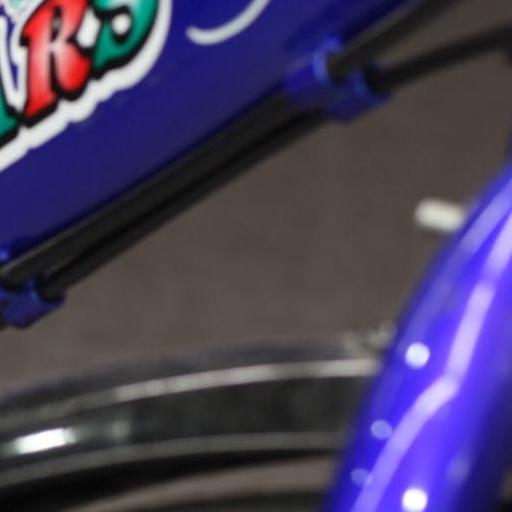
\includegraphics[scale=0.34]{assets/BlueMean.JPG}
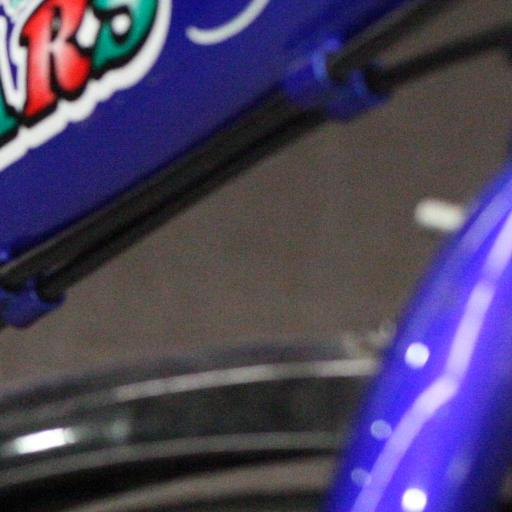
\includegraphics[scale=0.34]{assets/BlueReal.JPG}
\caption{Citra Ground Truth dan Asli Sepeda Biru \cite{xu2018realworld}}
\end{figure}

\begin{figure}[H]
\centering
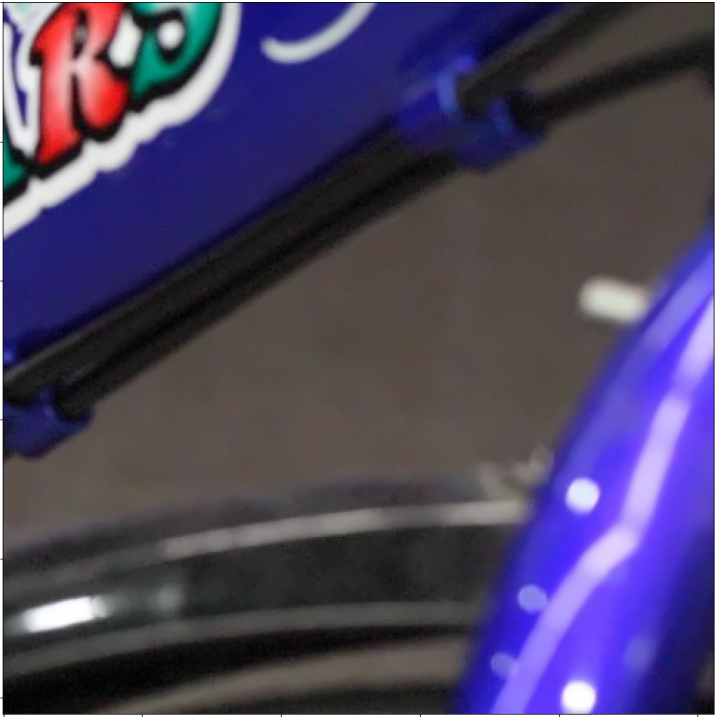
\includegraphics[scale=0.4]{assets/BlueNLMeans.png}
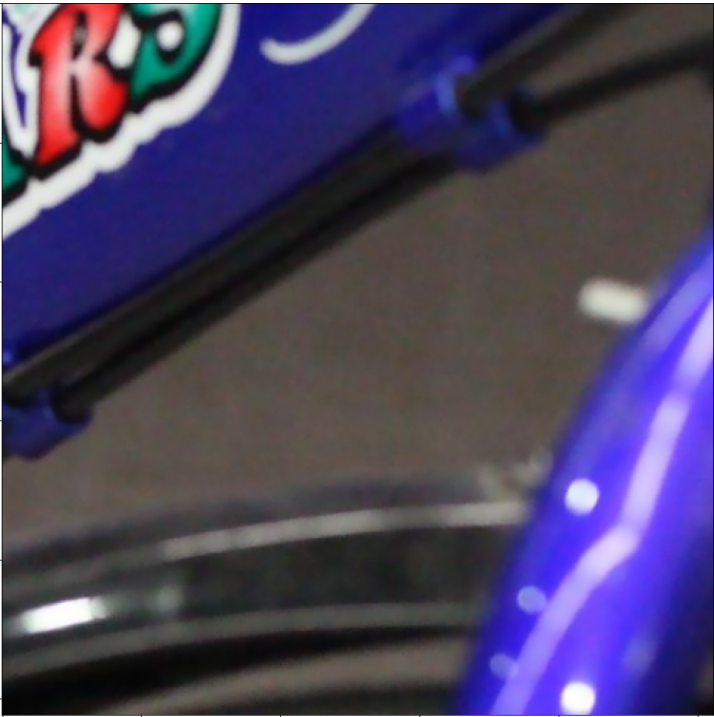
\includegraphics[scale=0.4]{assets/BlueGuided.png}
\caption{Non-Local Means dan Guided Filtering pada Sepeda Biru}
\end{figure}

Di dalam kasus ini, secara subjektif citra yang sebelah kiri terlihat melakukan \textit{denoising} dengan lebih baik. Hal ini memang karena adanya bagian segmen gambar yang lebih flat dan warnanya cenderung monoton. \textit{noise} yang terdapat pada bagian tersebut tidak bisa ter-\textit{blend} dengan rata dalam seluruh gambar (hanya jendela tertentu saja) pada citra hasil \textit{guided filtering} yang sebelah kanan.

\begin{figure}[H]
\centering
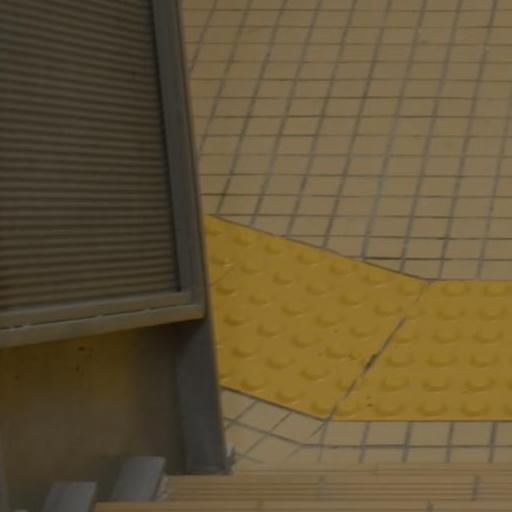
\includegraphics[scale=0.34]{assets/TanggaMean.JPG}
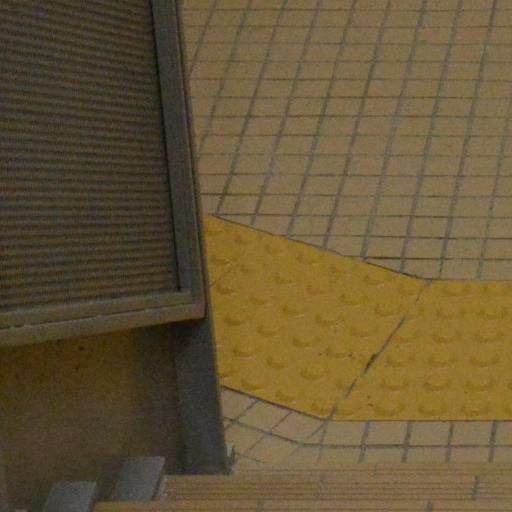
\includegraphics[scale=0.34]{assets/TanggaReal.JPG}
\caption{Citra Ground Truth dan Asli Tangga \cite{xu2018realworld}}
\end{figure}

\begin{figure}[H]
\centering
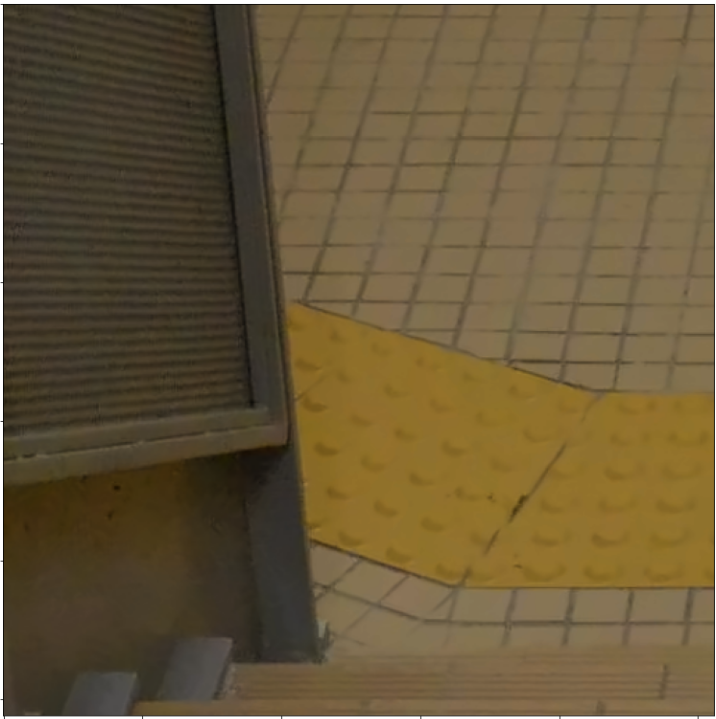
\includegraphics[scale=0.4]{assets/TanggaNLMeans.png}
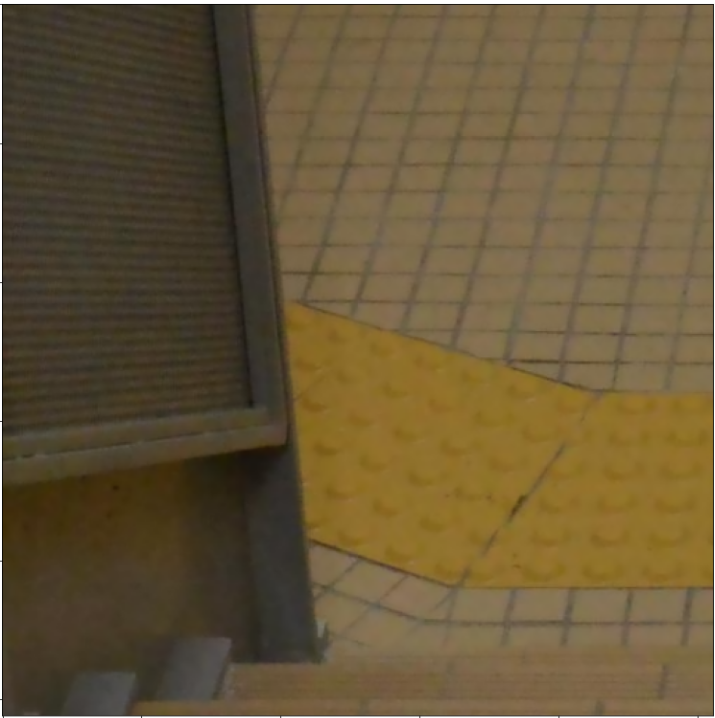
\includegraphics[scale=0.4]{assets/TanggaGuided.png}
\caption{Non-Local Means dan Guided Filtering pada Tangga}
\end{figure}

Dalam kasus ini, citra hasil \textit{non-local means filtering} tampak terlihat terlalu meratakan \textit{noise}, sehingga detail-detail penting seperti sisi ubin pada tangga juga ikut menghilang. Sehingga membuat Citra hasil \textit{guided-filtering} tampak lebih bagus. Begitu pula dengan beberapa kasus yang serupa untuk pola pada sofa dan detail debu pada kabel yang dihilangkan karena dianggap \textit{noise} oleh \textit{non-local means filtering}. Dalam kasus ini, juga menjadi dilema bagi mesin untuk menentukan mana \textit{noise} yang sesungguhnya dan mana yang merupakan detail dari sebuah gambar.

Untuk metode-metode \textit{deep learning}, hasilnya serupa dengan gambar \textit{ground truth}. Dari beberapa gambar, memang agak sulit dibedakan mana gambar yang merupakan \textit{ground truth} dan yang merupakan hasil inferensi menggunakan \textit{deep learning}. Beberapa alasan lain juga karena resolusi gambar yang memang terlalu kecil untuk bisa dinilai secara subjektif dan penuh.

\begin{figure}[H]
\centering
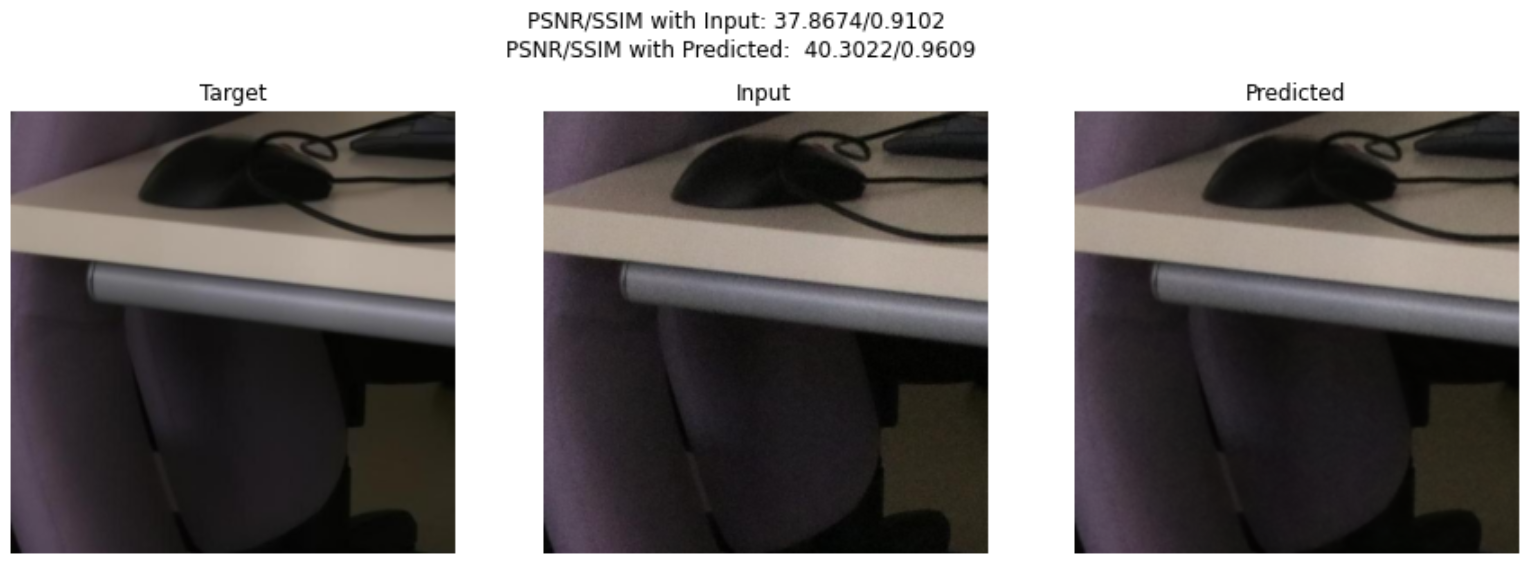
\includegraphics[scale=0.5]{assets/RestormerImage.png}
\caption{Hasil Inferensi Gambar menggunakan Restormer}
\end{figure}

Secara umum, metode \textit{deep learning} yang menggunakan Uformer dan Restormer lebih unggul daripada semua metode konvensional yang kami coba. Namun perlu diperhatikan pula waktu yang dibutuhkan untuk melatih kedua model \textit{deep learning} ini bisa sangat lama dan membutuhkan \textit{resource} yang sangat banyak.

\begin{table}[H]
\centering
\begin{tabular}{|c|c|c|c|c|}
\hline
Metode             & PSNR-Min    & PSNR-Max    & SSIM-Min   & SSIM-Max   \\ \hline
Baseline           & $32.334257$ & $41.003953$ & $0.829040$ & $0.969997$ \\ \hline
Bilateral          & $32.406467$ & $41.841309$ & $0.884197$ & $0.985104$ \\ \hline
NL Means           & $32.761859$ & $42.031446$ & $0.888428$ & $0.982137$ \\ \hline
Guided             & $32.919550$ & $42.848544$ & $0.898302$ & $0.983398$ \\ \hline
Uformer-baseline   & $32.112148$ & $43.342189$ & $0.916373$ & $0.984347$ \\ \hline
Uformer-tuned      & $33.607654$ & $44.580649$ & $0.922405$ & $0.989854$ \\ \hline
Restormer-baseline & $32.737102$ & $43.496461$ & $0.919680$ & $0.984807$ \\ \hline
Restormer-tuned    & $33.573822$ & $44.491641$ & $0.921844$ & $0.989544$ \\ \hline
\end{tabular}
    \caption{Minimum dan Maksimum Metriks Akurasi}
\end{table}

Bila diperhatikan pula dari nilai minimum dan maksimumnya, terlihat bahwa rata-rata dan nilai ekstremnya berbanding lurus terhadap hasil akurasi pula. Namun memang ini mengartikan adanya fluktuasi antara setiap gambar, tidak selalu memberikan hasil yang bagus sekali pula dalam berbagai kasus. Karena masih terdapat kasus-kasus yang nilai PSNR-Minnya sangat rendah. Persebarannya memang cukup \textit{skew left} bila kita perhatikan berdasarkan nilai ekstremnya saja. Namun secara keseluruhan, metode \textit{vision transformer} memang memberikan performa yang cukup timpang dengan metode konvensional.

\chapter{Penutup}

\section{Kesimpulan}

\textit{Noise} pada citra merupakan salah satu gangguan yang bisa mengurangi akurasi dalam melakukan \textit{image segmentation}, \textit{classification}, ataupun proses \textit{intermediate} dan \textit{high level processing}. Metode konvensional yang umumnya digunakan untuk melakukan restorasi citra yang memiliki \textit{noise} lebih praktis dan cenderung lebih cepat untuk memproses citra yang besar. Salah satu metode konvensional yang merupakan \textit{state-of-the-art} saat ini ialah \textit{guided filter} yang akurasinya bisa menyaingi metode-metode \textit{deep learning} biasa seperti \textit{convolutional neural network}, dan bahkan hanya memerlukan nilai rata-rata untuk suatu \textit{windows kernel} tertentu. 

Metode \textit{deep learning} yang dewasa ini sering digunakan ialah \textit{vision transformer} yang menggunakan metode \textit{self-attention} yang diadopsi dari metode-metode pemrosesan bahasa natural. \textit{Self-attention} ini merupakan mekanisme yang membolehkan melihat interaksi antar entitas dan \textit{feature maps} pada jaringan untuk mempelajari hierarki yang ada pada citra. Salah satu penerapannya ialah pada Uformer dan Restormer dalam melakukan \textit{image denoising}.

Berdasarkan akurasi, performa metode \textit{denoising} menggunakan \textit{vision transformer (deep learning)} menghasilkan citra yang lebih baik daripada metode konvensional yang ada saat ini. Namun, waktu yang dibutuhkan untuk melatih citra (\textit{precomputing}) relatif lebih lama, karena metode konvensional tidak membutuhkan ini. Metode \textit{deep learning} juga membutuhkan \textit{resource} yang jauh lebih banyak dan besar karena dalam praktiknya membutuhkan komputasi \textit{floating point} yang banyak untuk setiap iterasi dan validasinya. Setiap metode memiliki keunggulan dan kekurangannya, sehingga penggunaannya harus disesuaikan dengan sumber daya dan konteks dari \textit{image preprocessing} itu sendiri.

\section{Saran}

Dengan adanya hasil dari eksperimen ini, kami berharap pembaca dapat memahami cara kerja dan menentukan metode-metode \textit{image denoising} mana yang lebih sesuai untuk digunakan, berdasarkan hasil perbandingan akurasi, kecepatan, dan scalability dari metode-metode ini.

\section {Refleksi Kelompok}

Kami menemukan bahwa selain metode-metode \textit{smoothing} yang diajarkan di kelas pengolahan citra, ada berbagai metode lain dengan memanfaatkan berbagai properti lain dari citra pula. Metode ini bermacam-macam dan memiliki keunggulan dan kerugiannya. Kami juga jadi lebih memahami bagaimana perhitungan dan penurunan rumus untuk metode-metode seperti \textit{guided, bilateral,} dan \textit{non-local means filter}. Selain itu, kami juga lebih mengerti tentang \textit{deep learning} secara umum, terutama metode-metode terbaru yang merupakan \textit{state-of-the-art} dewasa ini yaitu \textit{vision transformer} yang serupa dengan \textit{transformer} pada pengolahan bahasa natural.

\newpage
\nocite{*}
\bibliographystyle{apalike}
\bibliography{bibliography.bib}
% \pagenumbering{gobble}

% \newpage
% \addcontentsline{toc}{chapter}{Lampiran}
% \chapter*{Lampiran}

\end{document}